\subsection{TorCoin Mining}

Mining TorCoin requires transferring bandwidth. We introduce a novel method of \textit{onion hashing} to prove end-to-end bandwidth transfer across a Tor circuit.

\begin{figure}[H]
  \centering
    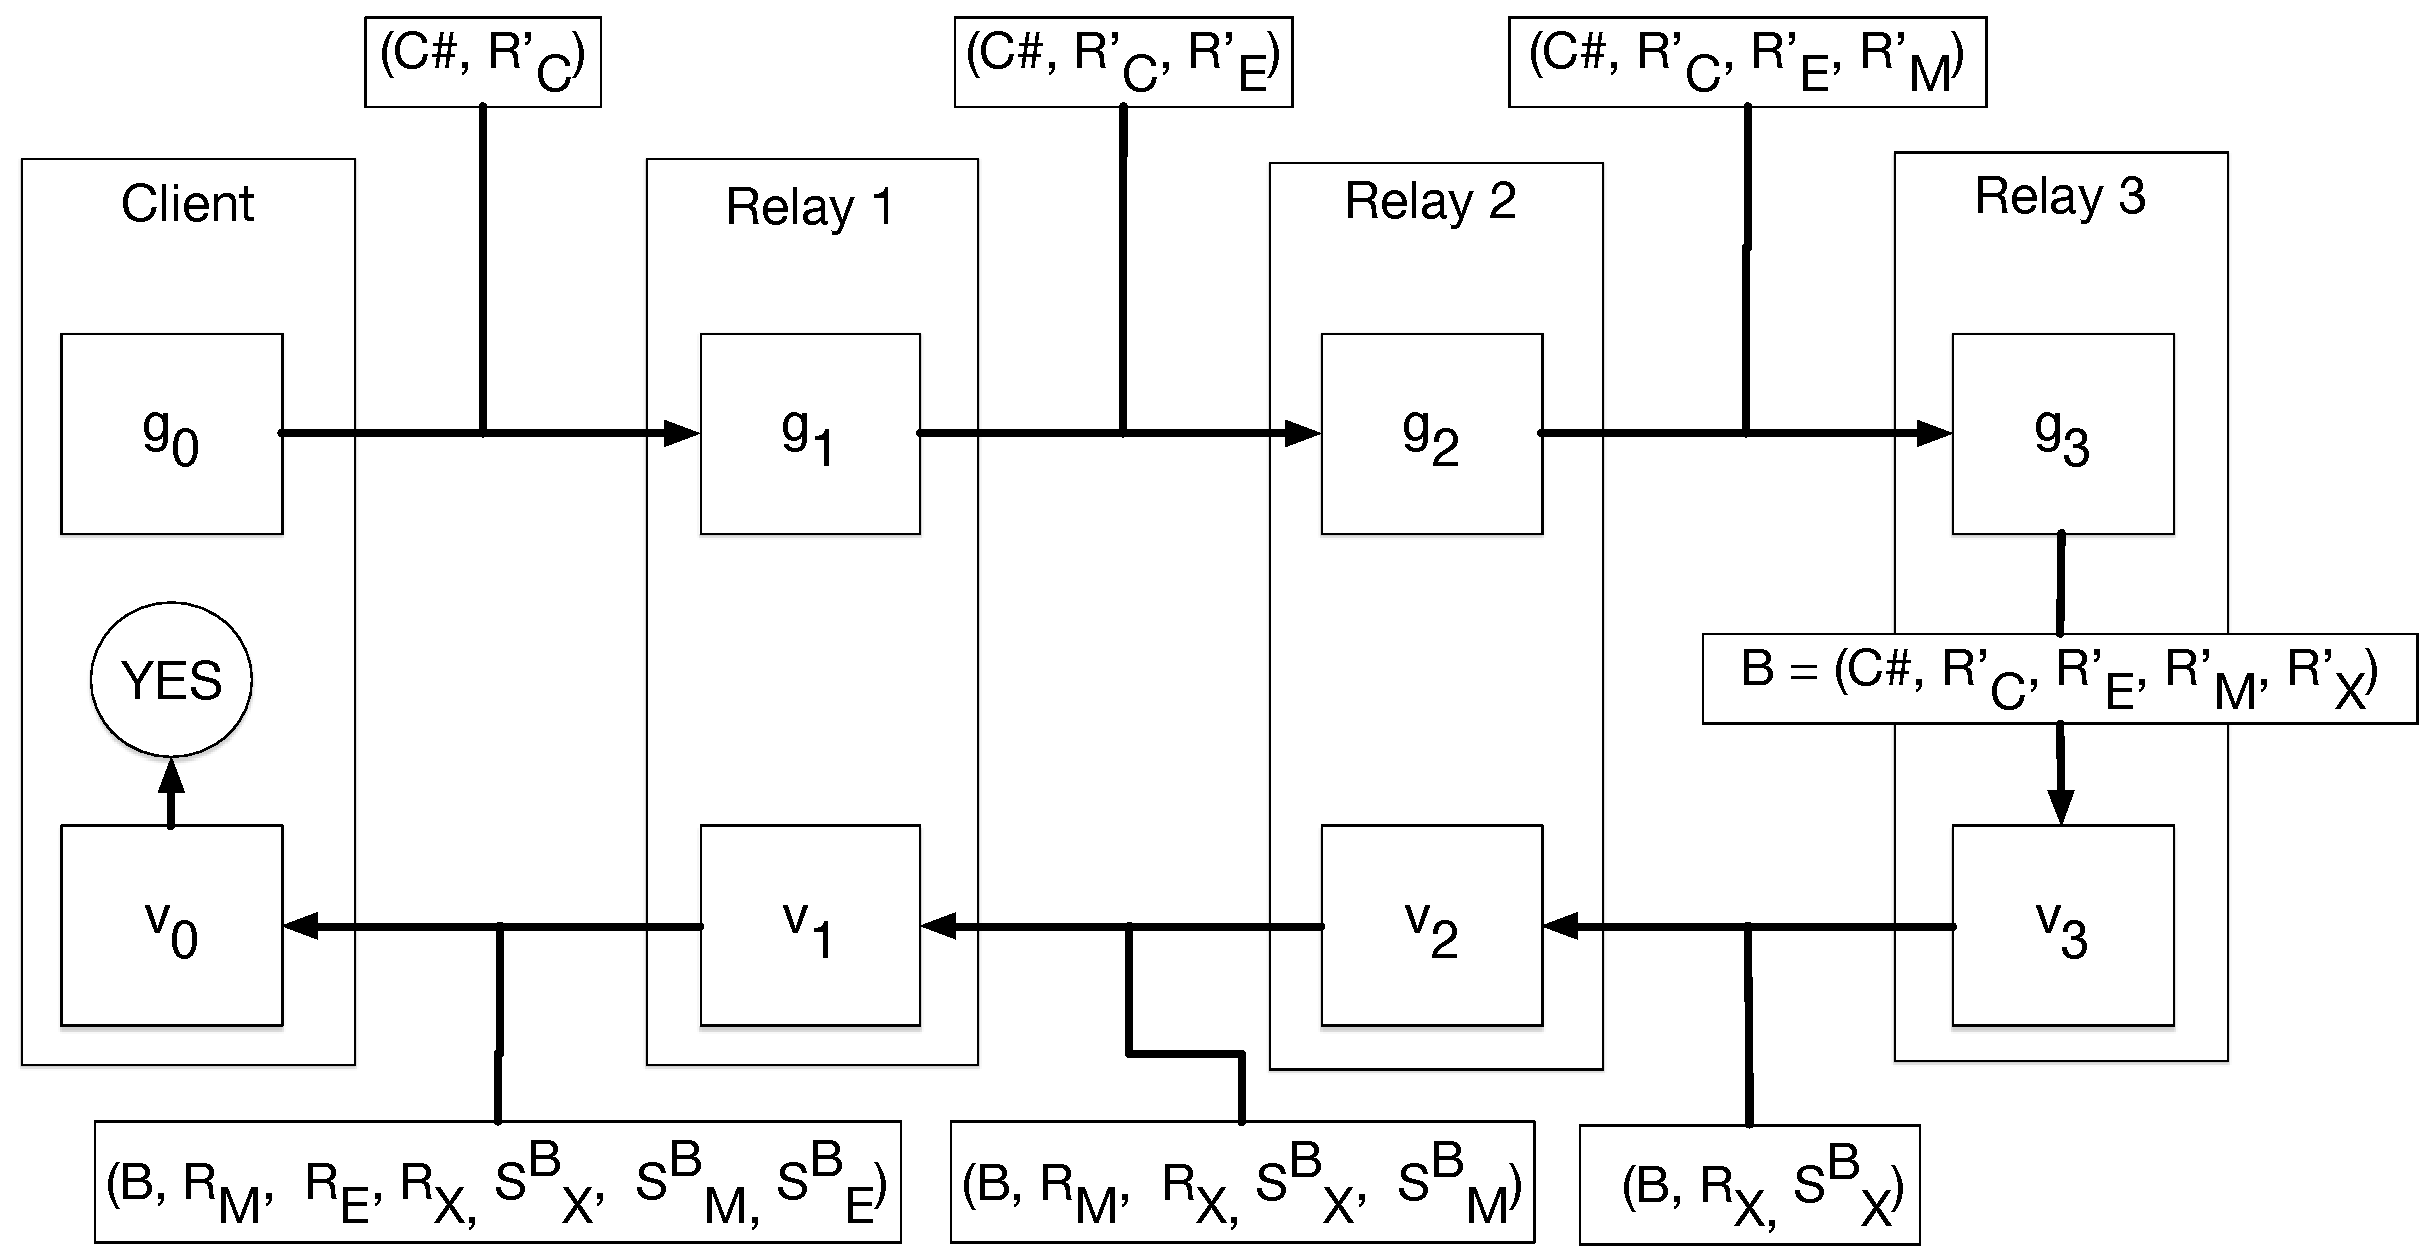
\includegraphics[scale=0.3]{torcoin_cycle.pdf}
  \caption{TorCoin Onion Hashing. Each circuit member has a generator and a verifier of hash wrappers. Here we represent private keys as distinct shapes.}
\end{figure}

\subsubsection{Onion Hashing Algorithm}
\begin{enumerate}
\item Every $m$ Tor packets, client sends a ``TorCoin packet'' containing a hash attempt $h_0$ likely to generate a TorCoin.
\item Relays pass $h_0$ ``around the circuit''
\subitem During $r_0 --> r_1 --> r_2$, the $h_0$ hash grows as each relay adds its own private key.
\subitem During $r_2 --> r_1 --> r_0$, the $h_0$ hash shrinks as each relay verifies the hash remained intact.
\item If client receives a hash wrapper containing the original $h_0$, it distributes $\frac{1}{3} TC$ to each circuit member.
\end{enumerate}

Formally:

\begin{verbatim}
Client sends to A: T0 (its hash attempt)
A sends to B     : Hash(T0 + K1) = Ta # K1 = A tmp priv key.
B sends to C     : Hash(Ta + K2) = Tb # K2 = B tmp priv key.
C computes       : Hash(Tb + K3) = Tc # K3 = C tmp priv key.
C sends to B     : (Tc, K3) to verify.
B sends to A     : (Tc, K3, Tb, K2) to verify.
A sends to client: (Tc, K3, Tb, K2, Ta, K1) to verify.
\end{verbatim}

\subsubsection{TorCoin}
We combine onion hashing with the BitCoin protocol to achieve TorCoin. Once the protocol mints a TorCoin, the TorCoin Wallet writes it to the blockchain, along with the following information:

\begin{itemize}
\item Timestamp of consensus group.
\item Public key of client.
\item Circuit signature.
\item TorCoin hash.
\end{itemize}

All the information necessary for verifying proof-of-bandwidth is in the blockchain. 

\subsection{Security Considerations}

\subsubsection{Random Group Selection}
The TorPath protocol increases robustness of TorCoin to attackers. Its random group selection system inhibits attackers from deterministically placing themselves in a group. We could make the system even more secure by randomizing group assignment, instead of just taking temporal locality to be the only criterion.

\subsubsection{Colluding to Form Circuits}
In addition, because the attacker needs to control all four components of a route to mint a TorCoin fraudulently, even if the adversaries control up to half the network, there is a probability of only $(\frac{1}{2})^4 = \frac{1}{16}$ that an adversary client gets a path of three colluding relays. In practice, gaining control of half of the entire Tor client and relay network is practically impossible. 

\subsection{Drawbacks}
The TorPath network is not backwards compatible with the existing Tor network, due to the fundamental differences of route assignment and access control, which are missing in Tor, but are necessary for the TorPath and TorCoin schemes to work.

However, our scheme does not preclude a given physical relay or server from running both services at the same time. They will, of course, only get paid for the TorCoin traffic. In time, we expect that a majority of the current Tor relay operators will switch over to the TorPath network, since TorPath has the same security guarantees as Tor provides, while also recompensing the relay operators for their costs.

Backwards-compatible Tor incentivization schemes like Tortoise\cite{acsac11-tortoise}, Gold Star\cite{incentives-fc10}, LIRA and Opportunistic Bandwidth measurement have all had significant drawbacks like the usage of Eigenspeed for bandwidth measurement or the establishment of a central bank to keep track of their tokens. These all introduce significant infrastructure into the Tor network and sometimes partition the anonymity sets